
\subsection{Plane-Based Intersection}

\label{sec:embed}
%Given a triangle face $t$, we first convert to its P-rep: a supporting plane $\bm{p}_{t, sp}$ surrounded by three bounding planes $\{\bm{p}_{t, b}^i|\ i = 0,1,2\}$. We integrate the plane-based geometry into each of the tree steps of M\"{o}ller's algorithm as following:

\begin{figure}[t]
\centering
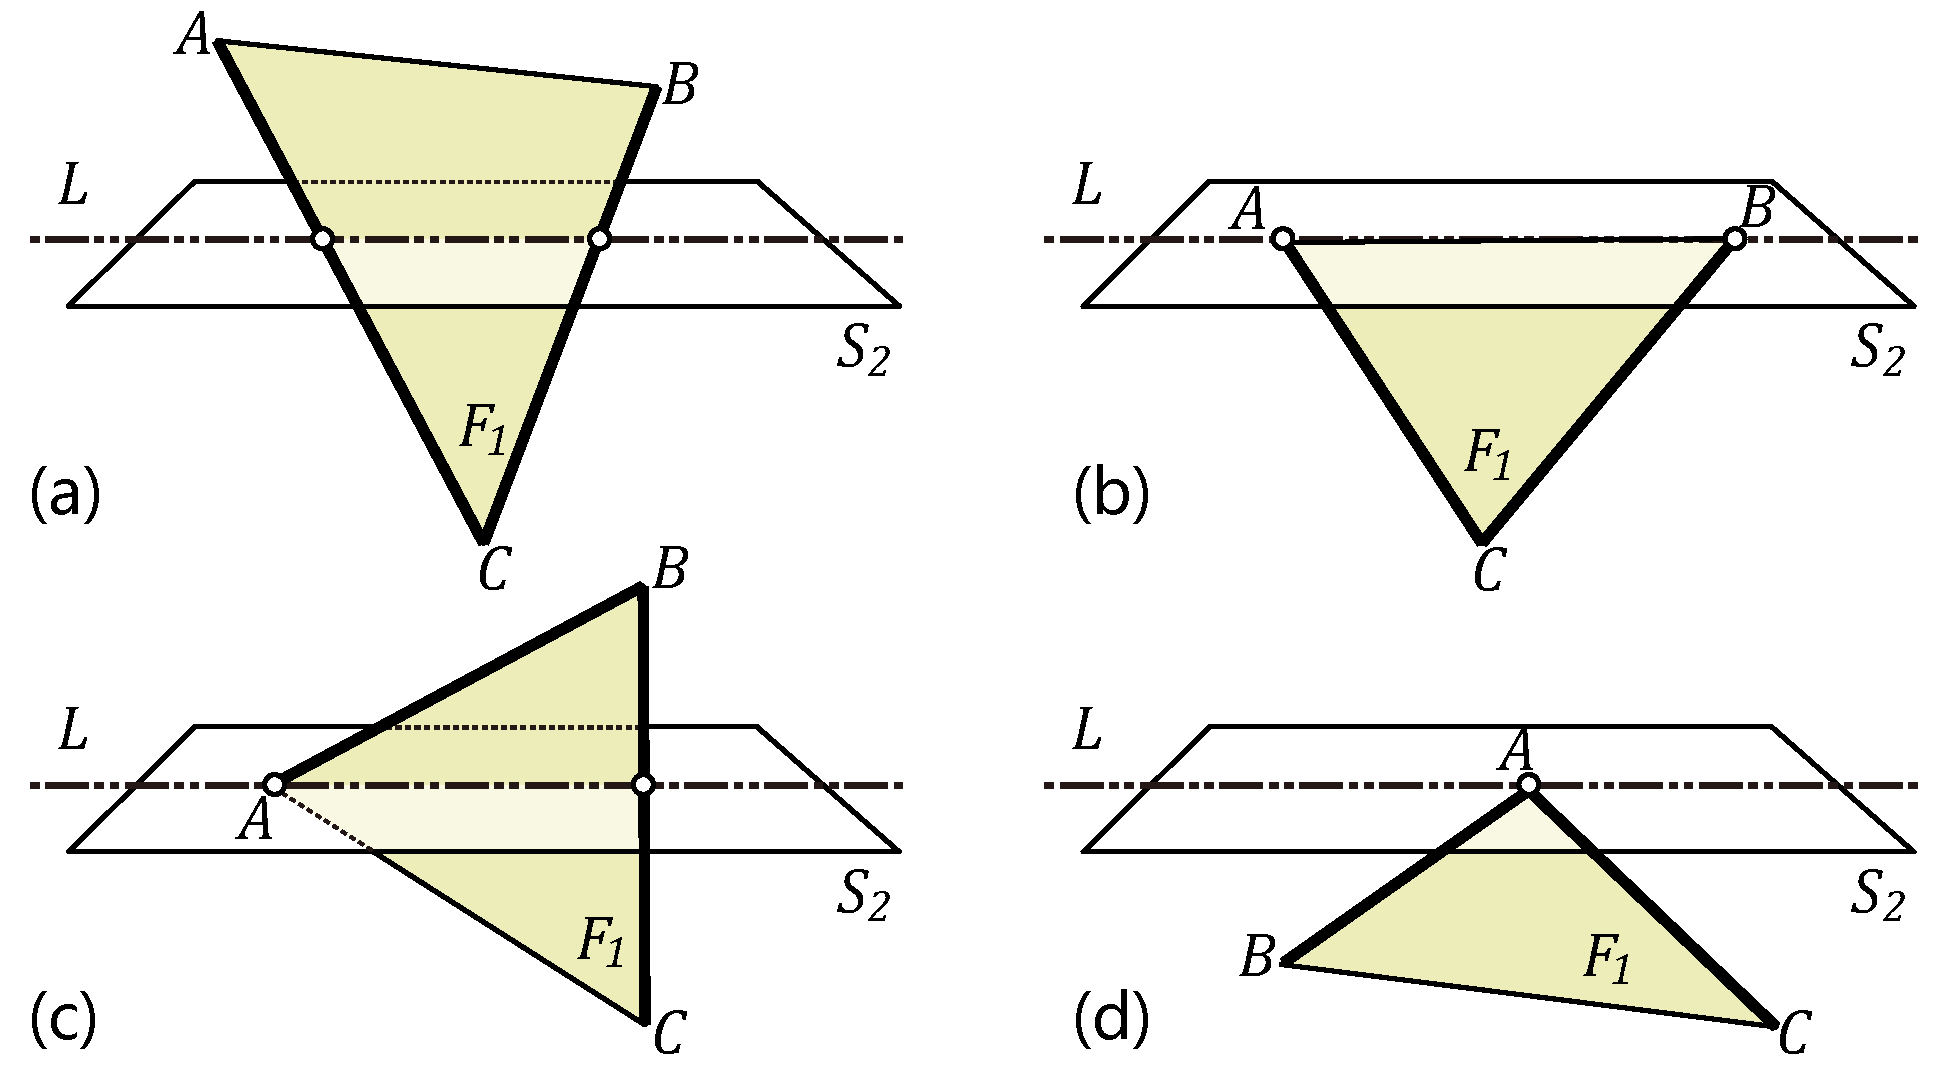
\includegraphics[width=3.5in]{sign}
\caption{We denote the signed distance from point $v_i$ to plane $\bm{p}_{t_2, sp}$ as $d_i$. The four conditions of intersection between $t_1$ and $\bm{p}_{t_2, sp}$ are:  (a) $d_0\cdot d_2<0$, $d_1\cdot d_2<0$; (b) $d_0=0$, $d_1=0$, $d_2\neq 0$; (c) $d_0=0$, $d_1\cdot d_2<0$; (d) $d_0=0$, $d_1\cdot d_2>0$. End points of $Seg_1$ are the intersections between $\bm{p}_{t_2, sp}$ and the related edges of $t_1$ (bold red lines).}
%We denote the signed distance from point vi to plane pt2,sp as di. The four conditions of intersection between t1 and pt2,sp are: (a) d0 �� d2 < 0, d1 �� d2 < 0; (b) d0 = 0, d1 = 0, d2 6= 0; (c) d0 = 0, d1 ��d2 < 0; (d) d0 = 0, d1 ��d2 > 0. End points of Seg1 are the intersections between pt2,sp and the related edges of t1 (bold red lines).
\label{fig:isect}
\end{figure}


Given a triangle face $t$, we first convert it to its P-rep: a supporting plane $\bm{p}_{t, sp}$  surrounded by three bounding planes $\{\bm{p}_{t, b}^i|\ i = 0,1,2\}$. We integrate the plane-based geometry into each of the three steps of M\"{o}ller��s algorithm as follows.
\begin{itemize}[leftmargin=0.45cm]
  %\item[1)] The basic subroutine of the first step is to compute the orientation of of a face with respect to vertices of the other face. We find that since the exact coordinates of each triangle vertices are known, we can compute the point-plane orientation using vertex-based geometry predicates. This allow us to perform this early rejection efficiently.
  \item[1)] The first step is to compute the orientation of a face with respect to the vertices of its paired face. As the exact coordinates of the vertices of each triangle are known, we can compute the point-plane orientation using vertex-based geometric predicates. This allows us to perform this early rejection efficiently.
      \vspace{0.5em}
  \item[2)] If $t_1$ and $t_2$ are not coplanar, the end points of $Seg_1$ and $Seg_2$ can be implicitly represented by plane triples. For example, $Seg_1$ is the intersection between $t_1$ and $\bm{p}_{t_2, sp}$ and the end points of $Seg_1$ are the intersections between $\bm{p}_{t_2, sp}$ and the edges of $t_1$ (denoted as $\bm{e}^i_{t_1}, i\in\{0,1,2\}$). Because $\bm{e}^i_{t_1}$ can be represented as $\bm{p}_{t_1, s}\cap \bm{p}^i_{t_1, b}$, the end points of $Seg_1$ can be represented in the form $\bm{p}_{t_2, sp} \cap \bm{p}_{t_1, sp} \cap \bm{p}^i_{t_1, b}$. Fig. \ref{fig:isect} shows all of the possible intersections between $t_1$ and $\bm{p}_{t_2, sp}$ and the corresponding $\bm{e}^i_{t_1}$. The coplanar situation is discussed in \S \ref{sec:degenerate}.
      % 2)	If t1 and t2 are not coplanar, the end points of Seg1 and Seg2 can be implicitly represented by plane triples. For example, Seg1 is the intersection between t1 and pt2,sp, and
      \vspace{0.5em}
 \item[3)] The intersection between $t_1$ and $t_2$ is the overlap between of $Seg_1$ and $Seg_2$. It can be computed by sorting the end points of $Seg_1$ and $Seg_2$ along the line $\bm{l}\colon \bm{p}_{t_1, sp} \cap \bm{p}_{t_2, sp}$. Because end points are all represented using plane triples, we can use the linear order of points, discussed in \S \ref{sec:substrates}, to sort them.

     %3)	The intersection between t1 and t2 is the overlap between Seg1 and Seg2. It can be computed by sorting the
\end{itemize}

%Each time an intersection is computed, two intersections are generated (one for each triangle) and the newly generated vertices are added into meshes. To avoid repetitive vertices in the final result, we perform vertex repetition elimination in this step, merging coincident vertices even if they come from different input meshes. Because we use P-reps, the comparison of vertices is exact.

Each time an intersection is computed, two intersections are generated (one for each triangle), and the newly generated vertices are added into their respective meshes. To avoid repetitive vertices in the final result, we perform vertex repetition elimination in this step; merging coincident vertices even if they come from different input meshes. Because P-reps are used, the comparisons of the vertices are exact.

\subsection{Plane-Based Intersection Representation}
\label{sec:ir}

In our method, the intersection with triangle $t$ is stored as $\bm{\mathcal{I}}\colon\{T, \bm{P}_{ext}, (\bm{P}_0, \bm{P}_1), \mathcal{N}\}$. This is the plane-based intersection representation (PBI-rep,  see Fig. \ref{fig:pbi}). The first component, $T$, indicates which triangle $\bm{\mathcal{I}}$ lies on. $\bm{P}_{ext}$ indicates that $\bm{\mathcal{I}}$ lies on $\bm{P}_{ext}$, which also means that it lies on the line $\bm{p}_{t, sp} \cap \bm{P}_{ext}$. The two end points of $\bm{\mathcal{I}}$ are $\bm{p}_{t, sp} \cap \bm{P}_{ext}\cap\bm{P}_0$ and $\bm{p}_{t, sp} \cap \bm{P}_{ext}\cap\bm{P}_1$. The last component, $\mathcal{N}$, represents the neighborhood of the intersection $\bm{\mathcal{I}}$. It indicates that $\bm{\mathcal{I}}$ is the intersection of triangle $t$ with $\mathcal{N}$ from the other mesh, where $\mathcal{N}$ can be either a face, or a set of faces that share the same edges.

%In our method, the intersection with triangle t is stored as I: {T,Pext,(P0,P1),N}.

\begin{figure}[t]
\centering
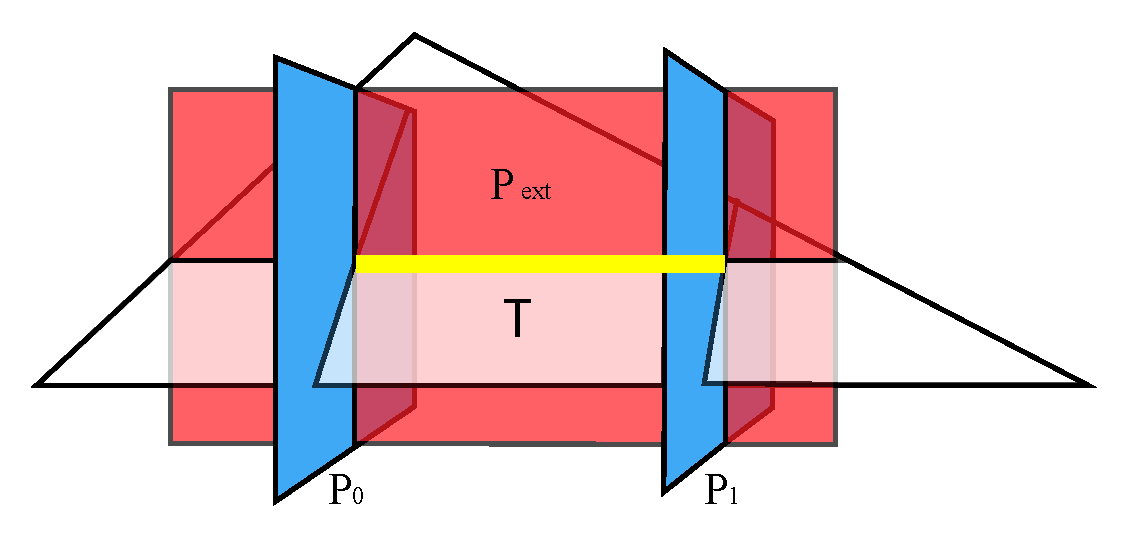
\includegraphics[width=3in]{pbirep2}
\caption{The geometry of planes in a PBI-rep. The yellow line segment is the intersection represented by $\bm{\mathcal{I}}$.}
\label{fig:pbi}
\end{figure}

%For example, two triangle faces $t_1$ and $t_2$ from mesh $M_i$ and $M_j$ intersect. Then it generates two intersections--- ${\bm{\mathcal{I}}}_{12}$ on $t_1$ and ${\bm{\mathcal{I}}}_{21}$ on $t_2$. For ${\bm{\mathcal{I}}}_{12}$ on $t_1$, $T = t_1$ and $\bm{P}_{ext}=\bm{p}_{t_2, sp}$. The third component is boundary planes from $t_2$ which has already been discussed in \S\ref{sec:embed}. The last component is $\mathcal{N}=t_2$. Sometimes intersections may lie on the mesh edges instead of faces (Fig. \ref{fig:twin}), which is called 'edge intersection'. In that case, the second component of neighborhood is a set of adjacent faces. We postpone the discussion of edge intersection to \S\ref{sec:degenerate}.

For example, two triangle faces, $t_1$ and $t_2$, originating from meshes $M_i$ and $M_j$, respectively, intersect. Two intersections are generated, ${\bm{\mathcal{I}}}_{12}$ on $t_1$ and ${\bm{\mathcal{I}}}_{21}$ on $t_2$. For ${\bm{\mathcal{I}}}_{12}$ on $t_1$, $T = t_1$ and $\bm{P}_{ext}=\bm{p}_{t_2, sp}$. The third component are the boundary planes of $t_2$, as discussed in \S\ref{sec:embed}. The last component is $\mathcal{N}=t_2$. Sometimes, intersections may lie on the mesh edges instead of their faces (Fig. \ref{fig:twin}). This is called ��edge intersection��. In this case, the second component is a set of adjacent faces. Edge intersection is discussed in \S\ref{sec:degenerate}.


\subsection{Handling Degenerate Case }
\label{sec:degenerate}

%While two triangles, if intersecting, intersect on a line segment in most situations, they can also intersect on a point or a convex area (coplanar case). Even if the intersection is a line segment, the intersection can be on triangle edges. These degenerate situations prevent us from performing robust boolean operations. In this section, we offer simple but effective way to deal with all these degenerations, which conceals the complexity of intersections and simplifies later processing.

In most situations, two intersecting triangles intersect on a line segment. However, they can also intersect on a point or a convex area (coplanar case). Even if the intersection is a line segment, the intersection can be on an edge. These degenerate situations prevent us from performing robust boolean operations. In this section, we demonstrate a simple but effective way of dealing with all of these degenerations, which conceals the complexity of intersections, and simplifies later processing.

%%%The criterion of whether an intersection help tessellation is by its necessity: if the intersection is not presented, whether some faces from the linked halfedge will cross the boundary of primitives. The word 'cross' do not only include the situation that a face is partly outside and partly inside of a primitive, but also can mean that a face is partly inside (outside) and part on the boundary of the primitive.


\subsubsection{Point intersection}
\label{sec:ipoint}
%If two triangles intersect on a single point (e.g., Fig. \ref{fig:isect}d), the intersection cannot be represented using our four-component description since the line segment collapses into a single point. In these cases, we simply add the intersection point into the related triangles to guarantee correct tessellation. No intersection is introduced.

If two triangles intersect at a single point (such as in Fig. \ref{fig:isect}d) then the intersection cannot be represented using our four-component description, because the line segment collapses into a single point. In these cases, we simply add the intersection point into the related triangles, which guarantees correct tessellation. No further intersections are introduced.

\subsubsection{Edge intersection}


%When intersection line segment lies on the edge of face, we call it \emph{edge intersection}. The space near edge intersection is divided by faces around the intersected edge (typically two faces for a manifold edge), instead of just one face. Therefore, the neighborhood of the related intersection is a set of faces instead of a single one. For example, in Fig. \ref{fig:twin}, the neighborhood of the intersection on $t_1$ is $\{t_2, t^*_2\}$.

When an intersecting line segment lies on the edge of a face, we refer to it as \emph{edge intersection}. The space near the edge intersection is divided by the faces around the intersected edge (typically two faces for a manifold edge), instead of by just one face. Therefore, the neighborhood of the corresponding intersection is a set of faces rather than a single face. For example, in Fig. \ref{fig:twin}, the neighborhood of the intersection on $t_1$ is $\{t_2, t^*_2\}$.

%Another thing needs to be noticed is that there will be repetitive detection of edge intersections. For example, in Fig. \ref{fig:twin}a, the same intersection on $t_1$ will be detected twice because $t_1$ intersect both $t_2$ and $t_2^*$ in exactly the same intersection. We solve this duplication together with other interactions among different intersections in \S\ref{sec:tessellation}. We also call such $t_2$ and $t_2^*$ as \emph{companion triangles} in an edge intersection because they share the same edge intersection. This concept will be referred again in the discussion of coplanar cases.

Edge intersections will be repeatedly detected. For example, in Fig. \ref{fig:twin}a, the same intersection on $t_1$ will be detected twice, because $t_1$ intersects both $t_2$ and $t_2^*$ at the same intersection. We solve this duplication, together with similar interactions between different intersections in \S\ref{sec:tessellation}. We regard $t_2$ and $t_2^*$ as \emph{companion triangles}, because they share the same edge intersection. This concept is referred to again in the discussion of coplanar cases.

\begin{figure}[t]
\centering
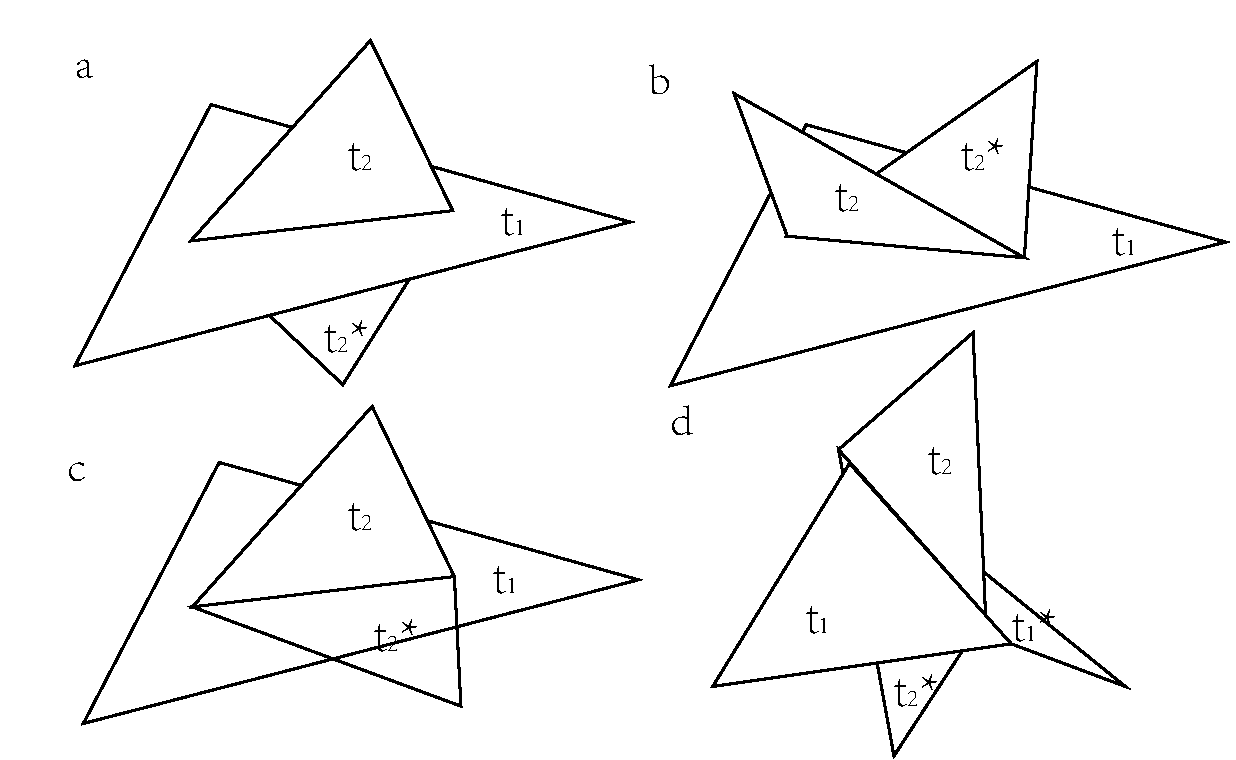
\includegraphics[width=3.5in]{edgeisect}
\caption{Different conditions of edge intersection. Triangle faces $t_1$ and $t_1^*$ are companion faces. Triangle faces $t_2$ and $t_2^*$ are companion faces. a) $t_2$ and $t_2^*$ are on different sides of $t_1$. b) $t_2$ and $t_2^*$ are on the same side of $t_1$. c) $t_2^*$ is coplanar with $t_1$. d) Both $t_1$ and $t_2$ have companion faces: the intersection is an edge intersection for both $t_1$ and $t_2$ (instead of only for $t_2$ is the previous three conditions). }
%Different conditions of edge intersection.
\label{fig:twin}
\end{figure}


\subsubsection{Copalnar}

\begin{figure}[t]
\centering
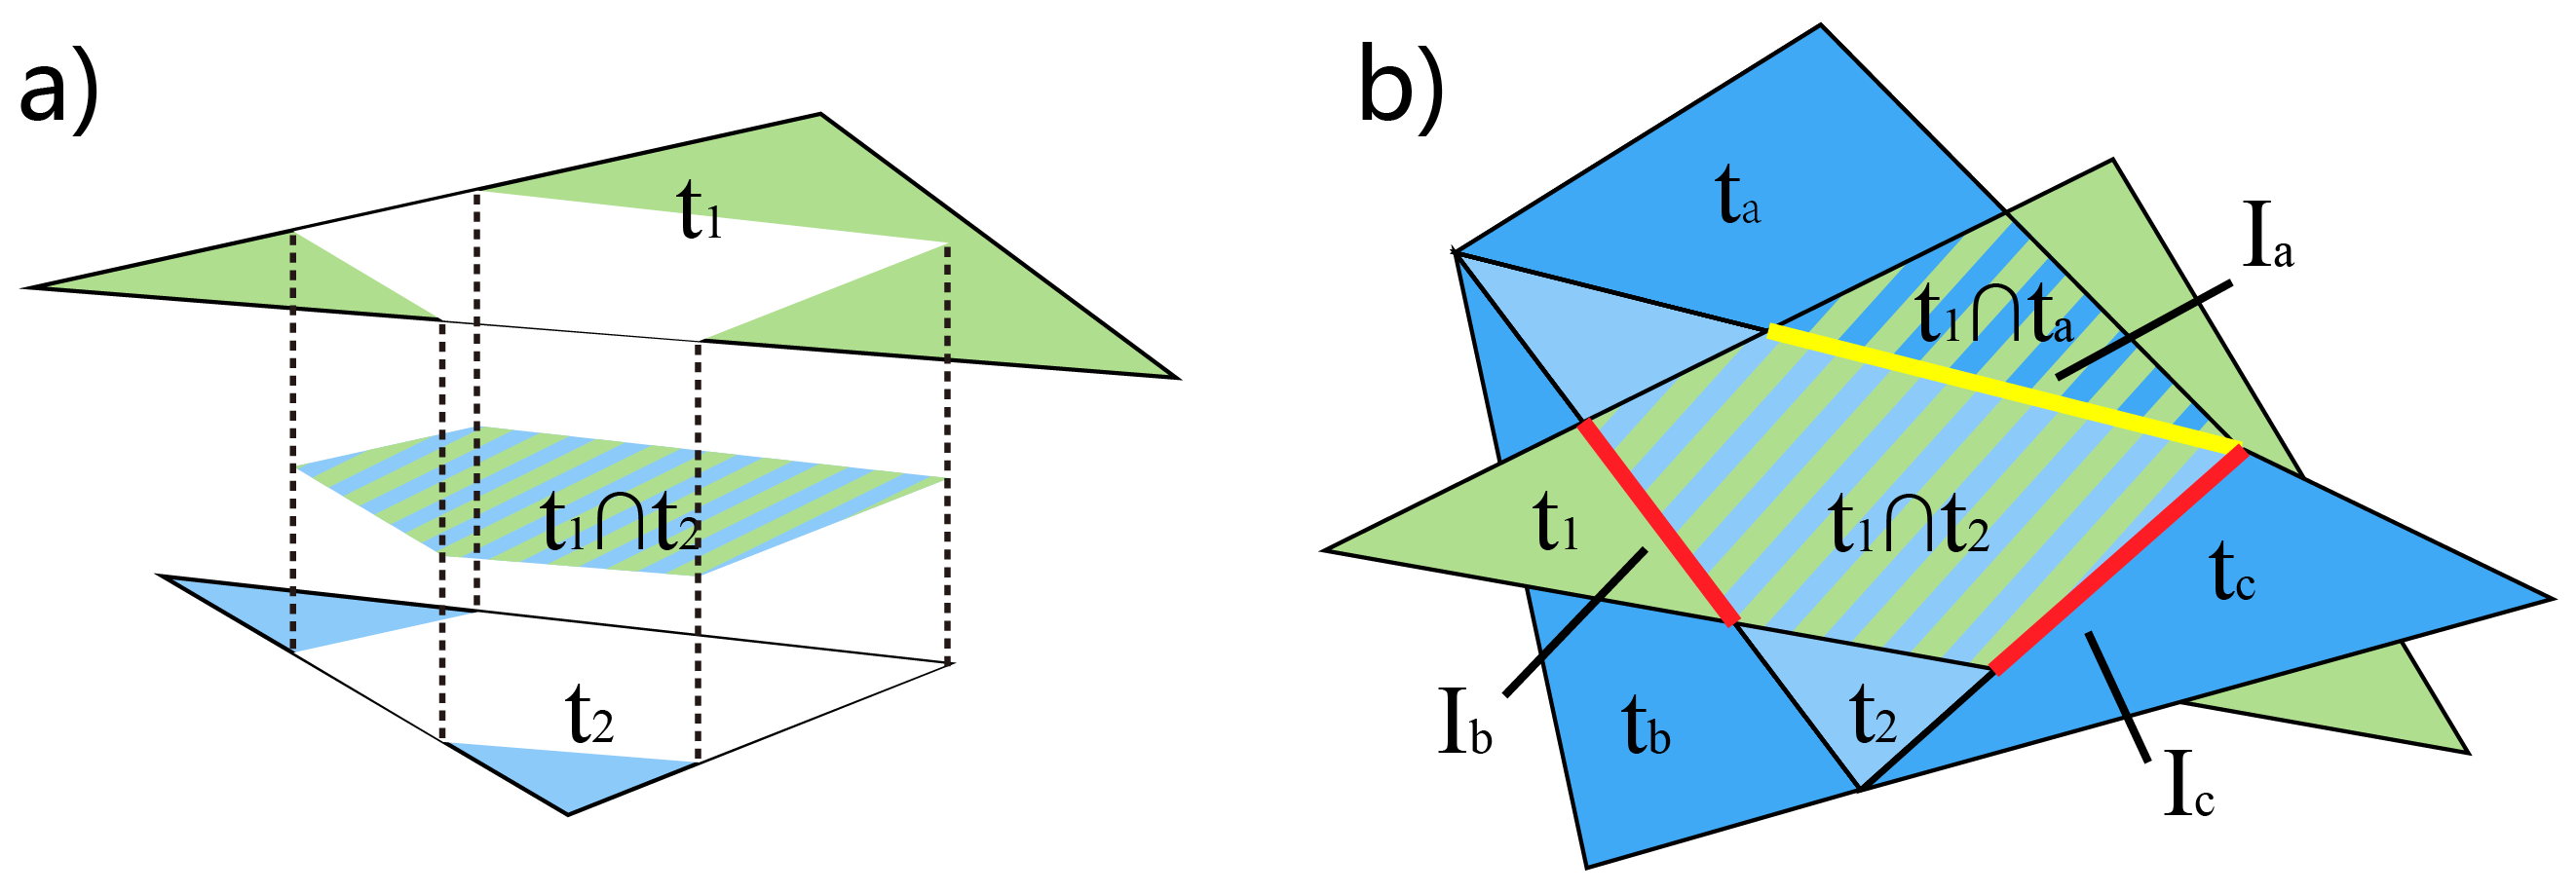
\includegraphics[width=3.5in]{boolean-03}
\caption{a) Coplanar cases; $t_1$ and $t_2$ intersect in 2D, dividing each other into two areas---a convex overlapping area and exclusive areas. b) Possible configurations of the companion faces. The blue triangles originate from the same mesh. For $\mathcal{I}_a$, the companion triangle $t_a$ is coplanar with $t_1$. Therefore, the overlapping areas ($t_1 \cap t_a$ and $t_1 \cap t_2$) do not need to be split by the yellow edge during tessellation, thus $\mathcal{I}_a$ is invalid. For $\mathcal{I}_b$ and $\mathcal{I}_c$, the companion faces are not coplanar, so these intersections can be recorded during an intersection test between $t_1$ and $t_a$ or $t_1$ and $t_b$. There is no need to record the intersection between $t_1$ and $t_2$.}
%Fig. 8. a) Coplanar cases; t1 and t2 intersect in 2D, dividing each other into two areas��a convex overlapping area, and exclusive areas.
\label{fig:coplanar}
\end{figure}

%Consider two triangle faces $t_1\in M_x$ and $t_2 \in M_y$ intersect within a common plane. Both $t_1$ and $t_2$ will divide each other into two areas---a convex overlapping area and exclusive parts (Fig. \ref{fig:coplanar}a). Apparantly, if we tessellate both $t_1$ and $t_2$ according to the boundary of overlapping area, we can guarantee that the tessellated meshes are intersection-free. Many previous methods \cite{feito2013fast,zhou2016mesh} use this method to guarantee topology correctness. However, in our method, we do not test whether $t_1$ and $t_2$ really intersect in 2D once we find they are coplanar. We treat coplanar situations as they do not intersect at all. In this way, we simplify our method, making it more robust and fast, while doing no harm to the topology correctness.

Consider two triangle faces,  $t_1\in M_x$ and $t_2 \in M_y$, which intersect within a common plane. Both $t_1$ and $t_2$ divide each other into two areas��a convex overlapping area and exclusive areas (Fig. \ref{fig:coplanar}a). If we tessellate both $t_1$ and $t_2$ according to the boundary of the overlapping area, we can guarantee that the tessellated meshes are intersection-free. Many previous methods \cite{feito2013fast,zhou2016mesh} use this process to guarantee topological correctness. However, in our method, we do not test whether $t_1$ and $t_2$ really intersect in 2D once we determine that they are coplanar. We treat coplanar situations as if they do not intersect at all. In this way, we simplify our method, making it faster and more robust, while having no effect on the topological correctness.

%We find that each intersection line segment in 2D is part of the edges from input meshes. That means we can view 2D intersection as a special case of edge intersection. The only difference is that there can be up to three edge intersections in one 2D intersection (red and yellow line segments in Fig. \ref{fig:coplanar}b). As we have discussed, edge intersection will be detected twice. That means we can rely on the companion triangle faces to detect intersections.

We find that each intersecting line segment is part of the edges of the input meshes in 2D. That means that we can view 2D intersections as special cases of edge intersections. However, there can be up to three edge intersections in one 2D intersection (red and yellow line segments in Fig. \ref{fig:coplanar}b). As discussed, edge intersections will be detected twice. Hence, we can rely on the faces of the companion triangles to detect intersections.

%However, if the companion triangles are also coplanar, neither of the two triangles will record the intersection. Fortunately, in this case, the intersection is not valid. The word `valid` means the intersections will appear as an edge in the final mesh, thus is necessary to put into tessellation. Supposing the intersection $\mathcal{I}$ is on $t_1$, this definition equals to:

However, if the companion triangles are also coplanar, neither of the two triangles will record the intersection. Fortunately, in this case the intersection is not valid. In this instance, ��valid�� means that it is necessary to tessellate the intersections, so that the intersections appear as an edge in the final mesh. Supposing the intersection $\mathcal{I}$ is on $t_1$, in which case:

\begin{equation}
% = f(\bm{\Lambda}(\bm{s}_i))
\lambda_f(\bm{v}_i) \neq constant, \bm{v}_i \in \bm{U}(\mathcal{I}) \cap M_x,
\end{equation}
.

%where f is the CSG function, and U(I) is the neighborhood of I in R3.
